\section{トラッカー部}
\label{implement_tracker}
トラッカー部の実装にはOpenCVを用いる.

QRコードの検出とデコードにはOpenCVに用意されているDetectQRクラスを利用し,そこから得られたQRコードの四角に対してPnPによる3次元再構成を行った.
PnPにはOpenCVに用意されているsolvePnPRansac関数を利用した.

これによりQRコードよりデコードされた次のQRコードの位置情報とQRコードに対するカメラの回転ベクトル,並進ベクトルが得られるのでこれらの情報をナビゲーション部\ref{implement_navigation}にて処理をする

実際にスマートフォン上に表示したQRコードに対して姿勢推定結果を描画したものを以下の図\ref{pnp_qr_img}に示す

\begin{figure}[htbp]
  \begin{center}
    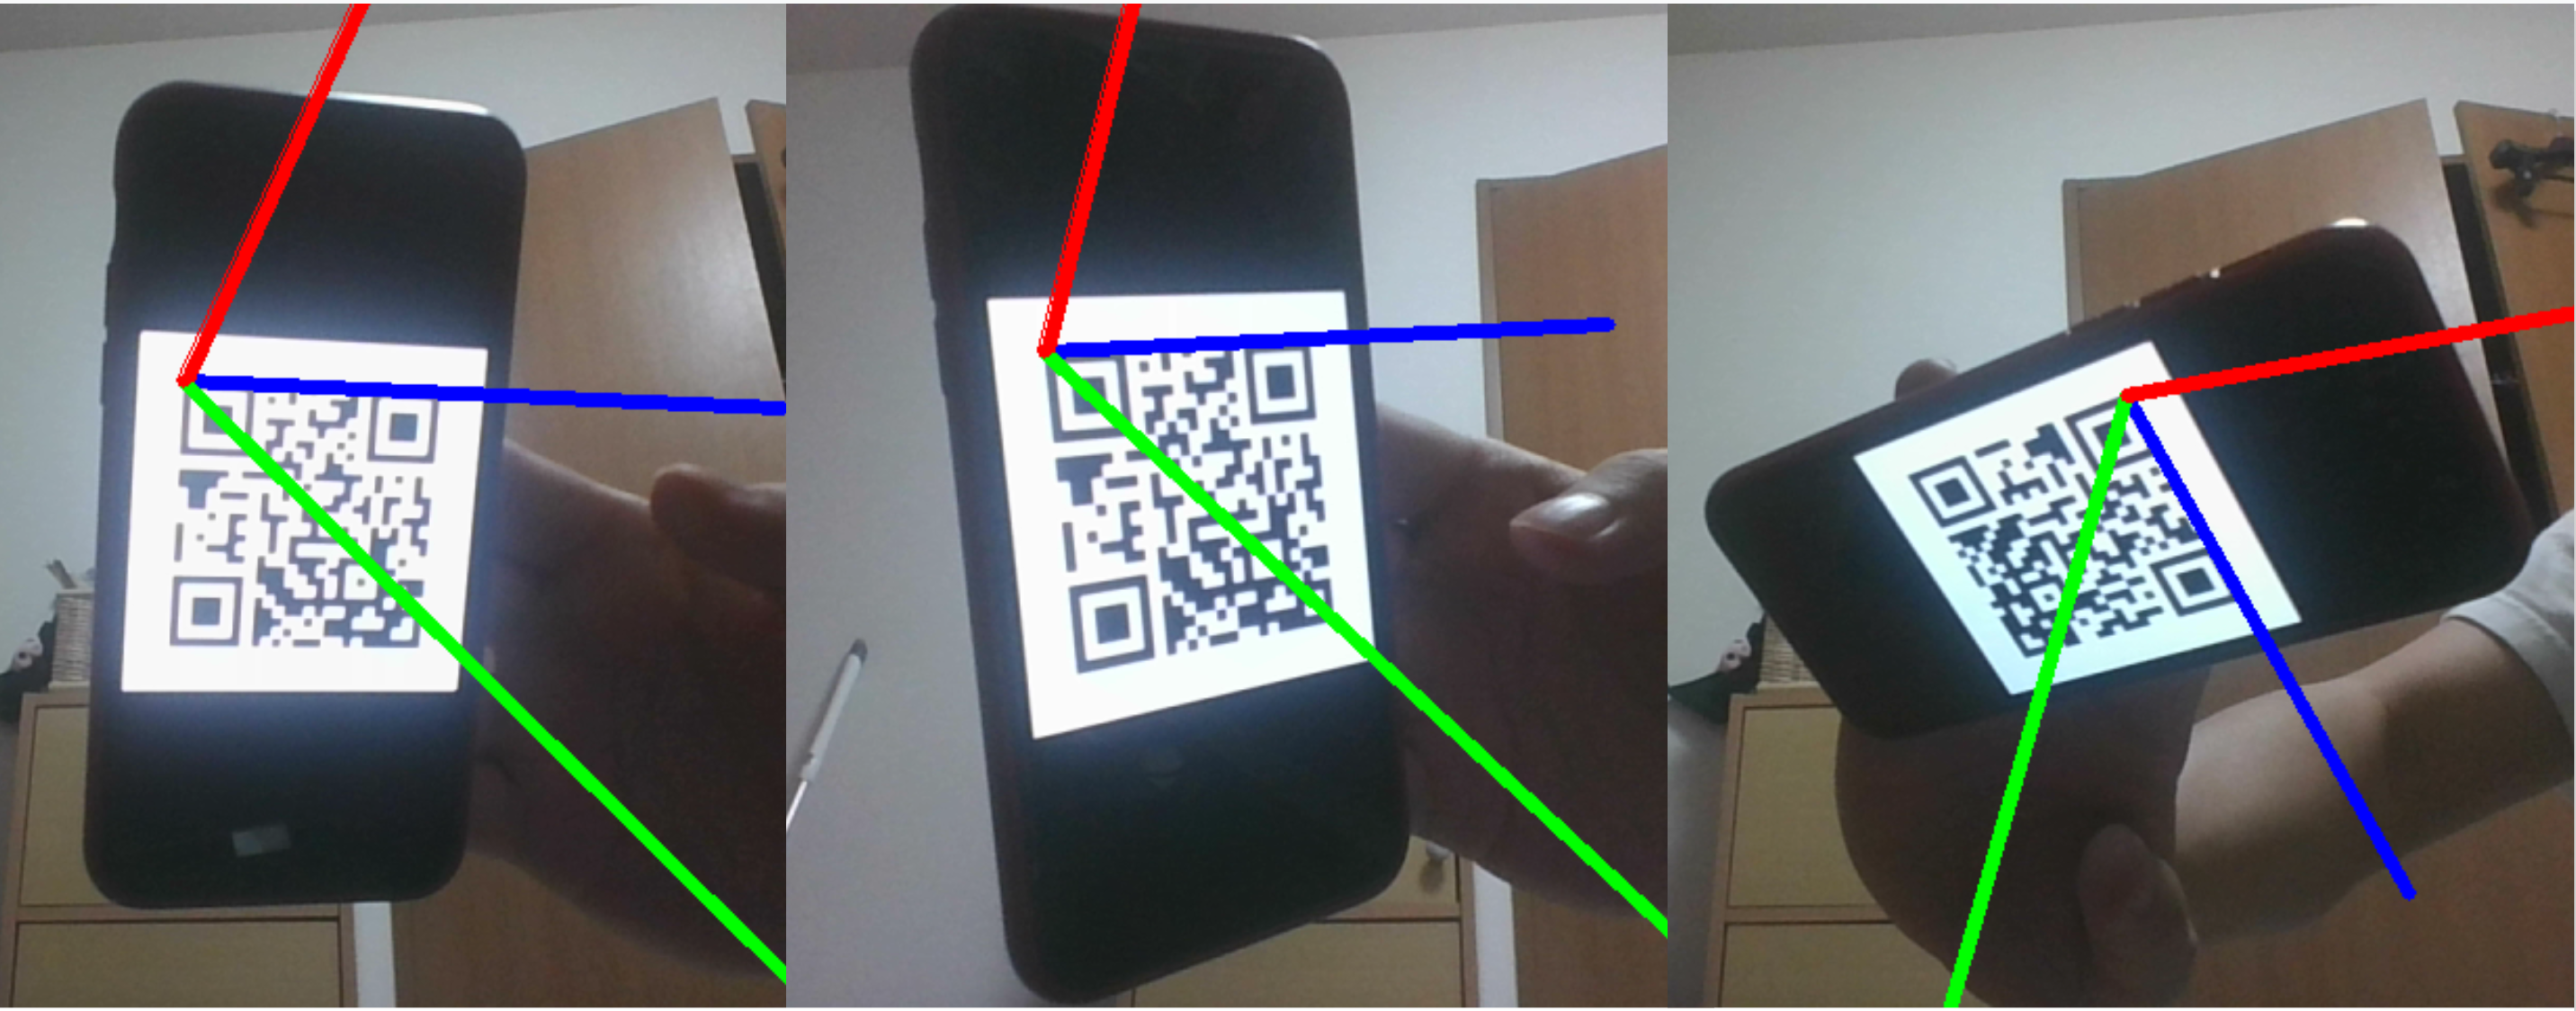
\includegraphics[clip,width=15.0cm]{img/pnp_qr.png}
    \caption{QRコードの姿勢推定結果}
    \label{pnp_qr_img}
  \end{center}
\end{figure}

ソースコードの該当部分をそれぞれ以下のプログラム\ref{src_pnp}に示す.
以下のプログラムでは映像からQRコードの検出,デコード,姿勢推定を行いバッファに推定値を追加している.
\begin{lstlisting}[caption=pnp method,label=src_pnp]
def pnp_qr(self, frame):                                                                                                                                     
    img = cv2.cvtColor(frame, cv2.COLOR_RGB2BGR)                                                                                                             
                                                                                                                                                             
    qr = cv2.QRCodeDetector()                                                                                                                                
    data, points, _ = qr.detectAndDecode(img)                                                                                                                
    if data:                                                                                                                                                 
        self.qr_data = self._qr_validator(json.loads(data))                                                                                                  
        _, origin_rvec, origin_tvec, inliers = cv2.solvePnPRansac(                                                                                           
            self.objp, points, self.mtx, self.dist)                                                                                                          
        if not self.is_moving:                                                                                                                               
            self.target_pos = self.qr_data                                                                                                                   
            tvec = origin_tvec * self.UNIT_SIZE                                                                                                              
            rvec = origin_rvec * self.RAD_UNIT                                                                                                               
            self.drone_pos_list.append(tvec)                                                                                                                 
            self.drone_rotate_list.append(rvec)                                                                                                              
            if len(self.drone_pos_list) > 20:                                                                                                                
                self.drone_pos_list.pop(0)                                                                                                                   
                self.drone_rotate_list.pop(0)                                                                                                                
            drone_avg_pos = np.mean(self.drone_pos_list, axis=(0))                                                                                           
            drone_avg_rotate = np.mean(self.drone_rotate_list, axis=(0))                                                                                     
            self.drone_pos = {                                                                                                                               
                'x': drone_avg_pos[0],                                                                                                                       
                'y': drone_avg_pos[1],                                      
                'z': drone_avg_pos[2],                                      
                'r': drone_avg_rotate[1]                                    
            }                                                               
        imgpts, jac = cv2.projectPoints(                                    
            self.axis, origin_rvec, origin_tvec, self.mtx, self.dist)       
        img = self.draw(img, points, imgpts)                                
                                                                            
        cv2.imshow('img', img)                                              
        cv2.waitKey(10)                                                     
    else:                                                                   
        cv2.imshow('img', img)                                              
        cv2.waitKey(10)                                                     
    if not self.count in self.log_data:                                     
        self.log_data[self.count] = time.time()                             
    self.out.write(img)    
\end{lstlisting}
